\documentclass{article}

\usepackage{graphicx, xcolor}
\usepackage{amsmath, amssymb}
\usepackage{float}
\usepackage{enumitem}
\usepackage[colorlinks=true,allcolors=blue]{hyperref}

\usepackage[margin=1in]{geometry}

\def\hwtitle{Homework 10: Laplace equation}
\def\hwauthor{Caden Gobat}
\def\hwdate{\today}

\usepackage{fancyhdr}
\lhead{\hwauthor}
\chead{\hwtitle}
\rhead{\hwdate}
\lfoot{\hwauthor}
\cfoot{}
\rfoot{\thepage}
\renewcommand{\footrulewidth}{0.4pt}
\pagestyle{fancy}

\author{\hwauthor}
\title{\hwtitle}
\date{\hwdate}

\begin{document}

\maketitle
\thispagestyle{fancy}

\section{Introduction}

In this final assignment, we solve the Laplace equation using the Gauss-Seidel method. The Laplace equation is a partial differential equation that governs the steady-state

\section{Results}

\bigskip
\noindent{\bf Question 1}
\medskip

We can approximate this by first representing the edges in polar coordinates. The central pipe has a radius of 10 cm, and can thus be represented simply by $r(\theta) = 10$. We will use only the upper quarter arc, as it is the same for all four sides of the square. We can represent the top edge of the square (side length 30 cm) using the formula $r(\theta)=\frac{15}{\sin\theta}$, with both of these functions on the domain $\frac{\pi}{4}\leq \theta \leq \frac{3\pi}{4}$. This means the distance between the two on this domain as a function of angle is $d(\theta)=\frac{15}{\sin\theta}-10$. We can integrate this and divide by the width of the domain to find the average: \begin{gather*}
    \int_{\pi\over 4}^{3\pi\over 4} \left(\frac{15}{\sin\theta}-10\right)d\theta \cong 10.73 \\
    \langle d \rangle \cong 10.73\left/\frac{\pi}{2}\right. \cong 6.83\text{ cm}
\end{gather*}

The temperature differential between the center and the edge is 200 K. Therefore, if the gradient were constant, we would expect it to have a value of $\displaystyle \frac{200\text{ K}}{6.83\text{ cm}}=29.27\text{ K/cm}$.

We can the calculate the power loss as \begin{align*}
    P &= -t\sigma \cdot \oint d\mathbf{l}_\perp \cdot \nabla T \\
    &= -(1\text{ cm})(10\text{ W/m/K}) \cdot 2\pi r_\text{contour} \cdot (29.7\text{ K/cm}) \\
    &\approx \boxed{-190\text{ W}}
\end{align*}

\newpage

\bigskip
\noindent{\bf Question 2}
\medskip

\begin{enumerate}[label=\alph*)]
    \item $ $ \begin{figure}[H]
        \centering
        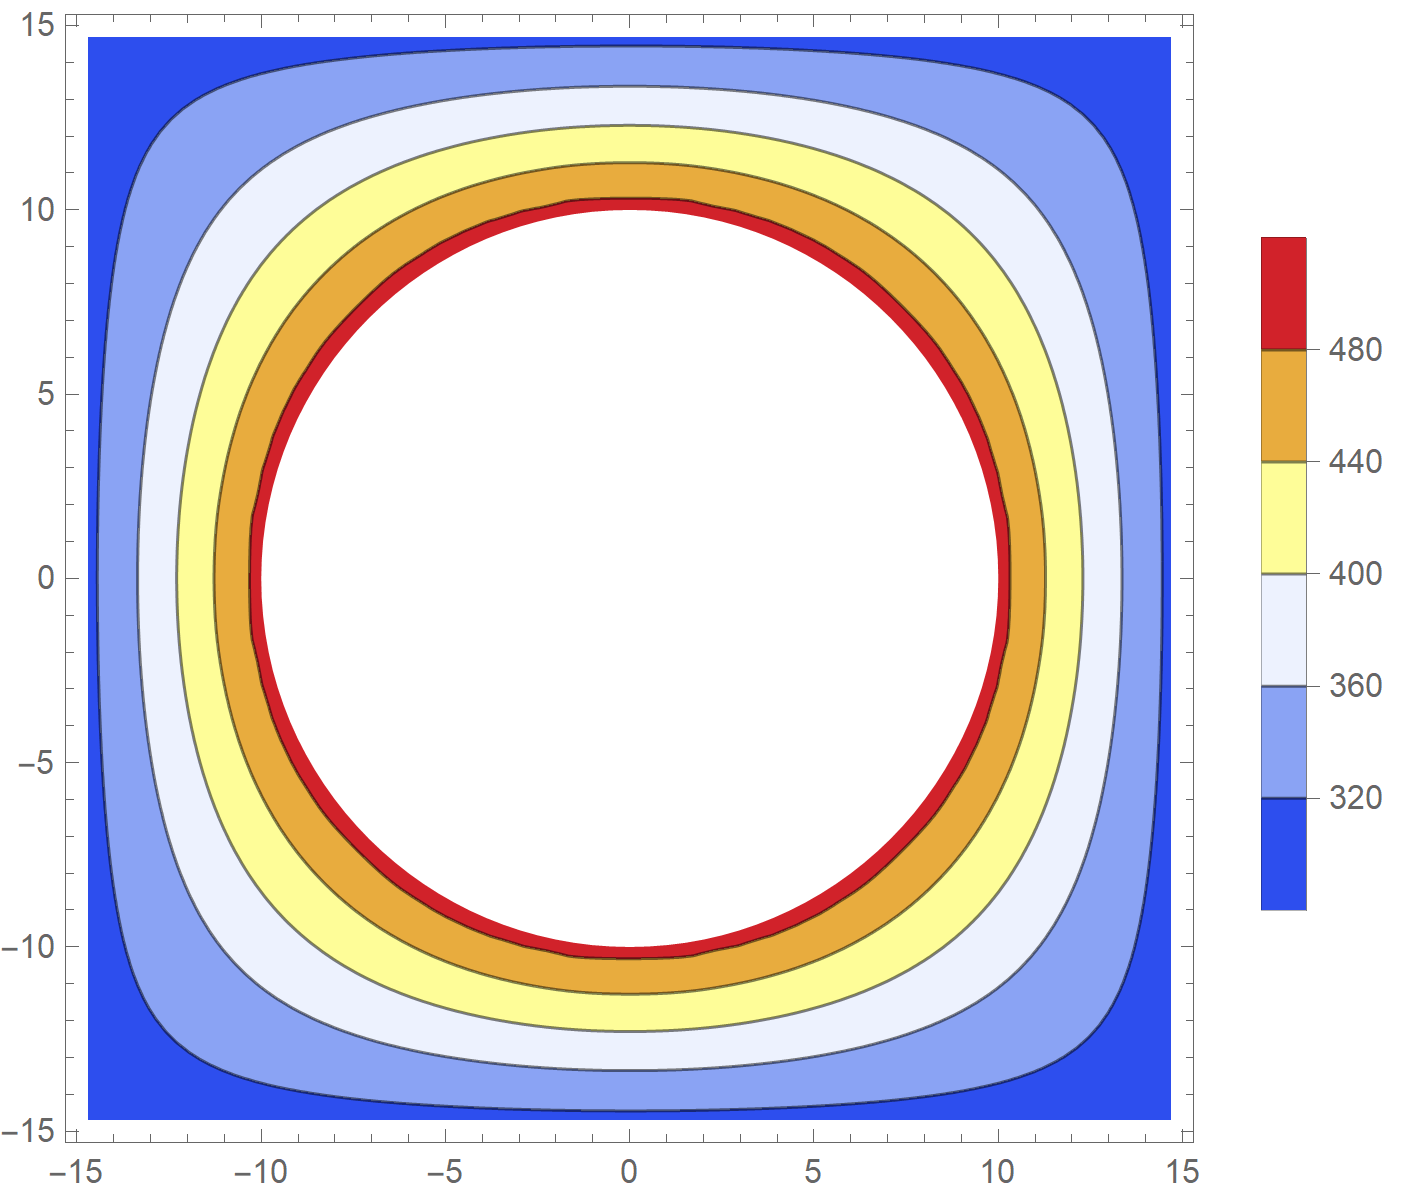
\includegraphics[width=5in]{homework10/2a.png}
        \caption{Contour plot of temperature through the square support plate.}
        \label{fig:2a}
    \end{figure}
    \item Heat flux has units of power per area. Because there is no loss, the flux through any closed contour on the support will be the same---the energy can't go anywhere else. First lets calculate the flux through the smaller contour (square circumscribing the pipe). I will use one side (here, the upper side, just above the circle in the $y$-direction), since the flux through each side of the square contour will be identical: \begin{align*}
        F &= \frac{\sigma}{A} \int_0^t\int_{\ell_\text{min}}^{\ell_\text{max}} \nabla T_y\ dx dh\\
        &= \frac{0.1\text{ W/(cm}\cdot\text{K)}}{10\text{ cm}^2}\cdot\int_0^1 \int_{-10}^{10} \nabla T_{y=10}\  dx dh \cong 637\text{ W/cm}^2
    \end{align*}
    Performing the same computation on the outside edge of the support yields \begin{gather*}
        F = \frac{0.1\text{ W/(cm}\cdot\text{K)}}{15\text{ cm}^2}\cdot\int_0^1 \int_{-15}^{15} \nabla T_{y=10}\  dx dh \cong 642\text{ W/cm}^2
    \end{gather*}
    These results are easily equivalent to within the margin of numerical/computation error, confirming that we have not incurred any unexpected losses.
    \newpage
    \item $ $ \begin{figure}[H]
        \centering
        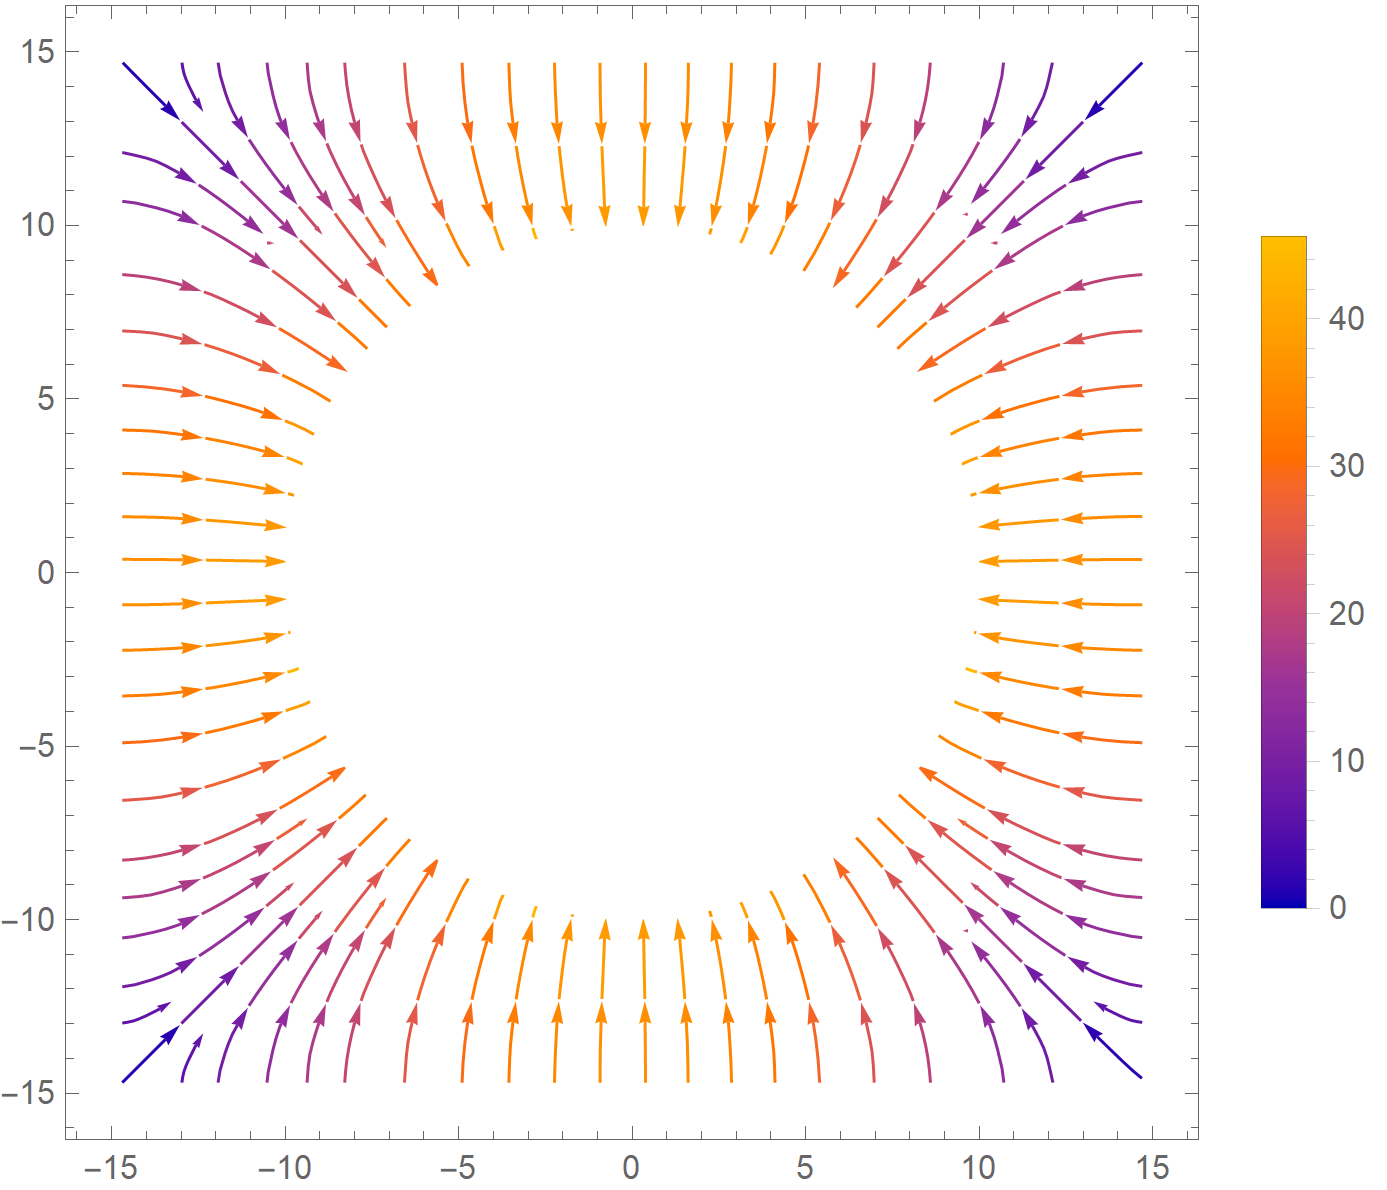
\includegraphics[width=5in]{homework10/2c.png}
        \caption{Temperature gradient throughout the support plate. Colors correspond to the magnitude of the gradient in K/cm.}
        \label{fig:2c}
    \end{figure}
\end{enumerate}

\bigskip
\noindent{\bf Question 3}
\medskip

\begin{figure}
    \centering
    \includegraphics{}
    \caption{Caption}
    \label{fig:3}
\end{figure}

\bigskip
\noindent{\bf Question 4}
\medskip

\begin{figure}
    \centering
    \includegraphics{}
    \caption{Caption}
    \label{fig:4}
\end{figure}

\section{Conclusions}

foo

\end{document}